\documentclass[dvipdfmx,tikz]{standalone}
\usepackage{tikz}
\begin{document}
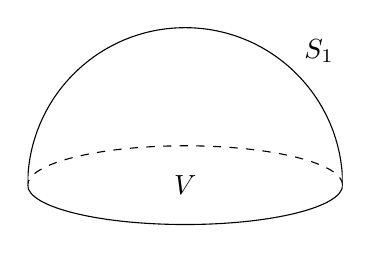
\begin{tikzpicture}
%\draw [help lines] (-2,-1) grid (2,2);
    \begin{scope}
        \clip (-2, 2) rectangle (2, 0);
        \draw circle [radius=2];
        \draw [dashed] circle [x radius = 2, y radius = 0.5];
    \end{scope}
    \begin{scope}
        \clip (-2, 0) rectangle (2, -0.7);
        \draw circle [x radius = 2, y radius = 0.5];
    \end{scope}
    \node {$V$};
    \node at (1.7, 1.7) {$S_1$};
\end{tikzpicture}
\end{document}